\section{گام پنجم: ترکیب خطی هرم‌ها (بخش ۴)}

در بخش ۲ دیدیم که استفاده از یک نقطه برش ثابت \lr{(Hard Cutoff)} برای ترکیب فرکانس‌ها، باعث ایجاد سایه‌های ناخواسته و پرش‌های ناگهانی در تصویر نهایی می‌شود. برای حل این مشکل، در این بخش از روش \textbf{ترکیب خطی \lr{(Linear Blending)}} استفاده می‌کنیم تا انتقال بین دامنه‌های فرکانسی به صورت کاملاً نرم و تدریجی انجام شود.

\begin{stepbox}
\field{منطق ترکیب خطی (وزن‌دهی تدریجی)}{
در این حالت، هیچ لایه‌ای به طور کامل به یک تصویر اختصاص داده نمی‌شود؛ بلکه لایه‌ی $i$ام هرم نهایی، ترکیبی وزن‌دار از لایه‌های $i$ام دو تصویر است. بر اساس صورت تمرین، وزن‌ها به شکل زیر تعریف می‌شوند:
\[ w_{\text{far}} = \frac{i-1}{7} \quad , \quad w_{\text{near}} = 1 - \frac{i-1}{7} \]
در این فرمول، هرچه به سمت لایه‌های بالاتر هرم (فرکانس‌های پایین‌تر) می‌رویم، سهم تصویر دور \lr{(Far)} بیشتر و سهم تصویر نزدیک \lr{(Near)} کمتر می‌شود.
}
\end{stepbox}

\subsection{پیاده‌سازی کد}
کد زیر نحوه محاسبه وزن‌ها و ترکیب لایه‌ها را نشان می‌دهد:

\begin{codebox}[\lr{Create Linear Hybrid Pyramid}]
\begin{lstlisting}[language=Python]
def create_linear_hybrid_pyramid(pyr_near, pyr_far):
    hybrid_pyr = []
    
    for j in range(8):
        weight_far = j / 7.0
        weight_near = 1.0 - weight_far
        
        hybrid_layer = (weight_near * pyr_near[j]) + (weight_far * pyr_far[j])
        hybrid_pyr.append(hybrid_layer)
        
    return hybrid_pyr
\end{lstlisting}
\end{codebox}

در پایتون، اندیس حلقه‌ی \lr{\texttt{for}} از ۰ تا ۷ است، بنابراین متغیر \lr{\texttt{j}} مستقیماً معادل عبارت $(i-1)$ در فرمول ریاضی صورت تمرین می‌باشد. لایه‌ی جدید (\lr{\texttt{hybrid\_layer}}) با ضرب هر لایه در وزن متناظرش محاسبه شده و به هرم اضافه می‌شود.

سپس این تابع را فراخوانی کرده و تصویر نهایی را بازیابی می‌کنیم:

\begin{codebox}[\lr{Execute and Build}]
\begin{lstlisting}[language=Python]
hybrid_linear_pyr_set1 = create_linear_hybrid_pyramid(pyr_near_set1, pyr_far_set1)
hybrid_linear_img_set1 = reconstruct_from_laplacian(hybrid_linear_pyr_set1)

comp_linear_hybrid_set1 = build_composite_pyramid(hybrid_linear_pyr_set1)

hybrid_linear_display = np.clip(hybrid_linear_img_set1, 0, 255).astype(np.uint8)
\end{lstlisting}
\end{codebox}

علاوه بر بازیابی تصویر اصلی، هرم لاپلاسی یکپارچه‌ی این حالت ترکیبی را نیز توسط تابع \lr{\texttt{build\_composite\_pyramid}} (که در بخش ۱ نوشتیم) تولید می‌کنیم.

\subsection{مقایسه خروجی‌ها و تحلیل نهایی}
در پایان تمرین پرسیده شده بود: \textbf{«تفاوت نتیجه این حالت با قسمت ۲ چیست؟»}

تفاوت اصلی حالت ترکیب خطی با حالت انتخاب گسسته \lr{(Hard Cutoff)} در \textbf{نرمیِ انتقالِ دامنه‌ی فرکانسی} است. در بخش ۲ به دلیل برش ناگهانی بین لایه‌ها، اثر شبح‌گون \lr{(Ghosting)} و تداخل خشن جزئیات روی هم دیده می‌شد. اما در ترکیب خطی، به دلیل تخصیص وزن‌های تدریجی، لبه‌های تصویر نزدیک به آرامی محو شده و جای خود را به سایه‌روشن‌های تصویر دور می‌دهند. در نتیجه، مرز انتقال فرکانس‌ها نامحسوس بوده و تصویر خروجی، به خصوص در نواحی میانی طیف فرکانسی، بسیار طبیعی‌تر و یکدست‌تر به نظر می‌رسد.

تصاویر زیر به خوبی گویای این تفاوت کیفیت هستند:

\begin{figure}[h!]
    \centering
    \begin{subfigure}{0.48\textwidth}
        \centering
        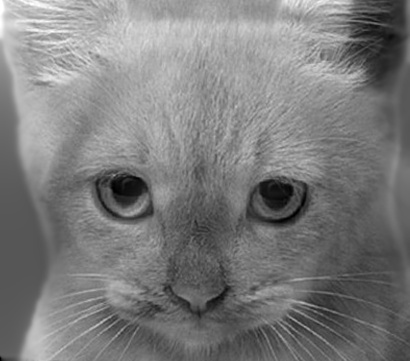
\includegraphics[width=\textwidth]{images/Hybrid_Linear_Set1.jpg}
        \caption{تصویر هیبریدی خطی (مجموعه حیوانات)}
    \end{subfigure}
    \hfill
    \begin{subfigure}{0.48\textwidth}
        \centering
        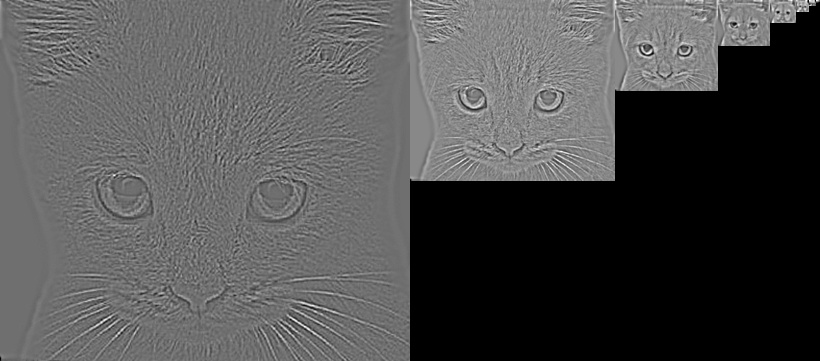
\includegraphics[width=\textwidth]{images/Laplacian_Pyramid_Linear_Set1.jpg}
        \caption{هرم لاپلاسی ترکیبی (مجموعه حیوانات)}
    \end{subfigure}
    
    \vspace{0.5cm}
    
    \begin{subfigure}{0.48\textwidth}
        \centering
        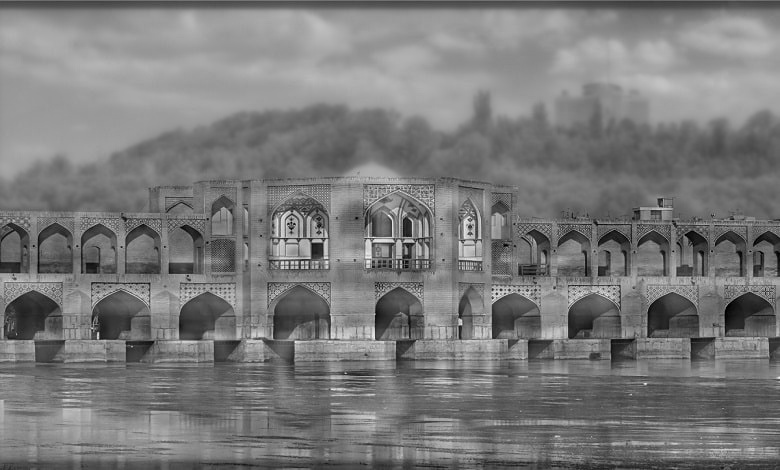
\includegraphics[width=\textwidth]{images/Hybrid_Linear_Set2.jpg}
        \caption{تصویر هیبریدی خطی (مجموعه بناها)}
    \end{subfigure}
    \hfill
    \begin{subfigure}{0.48\textwidth}
        \centering
        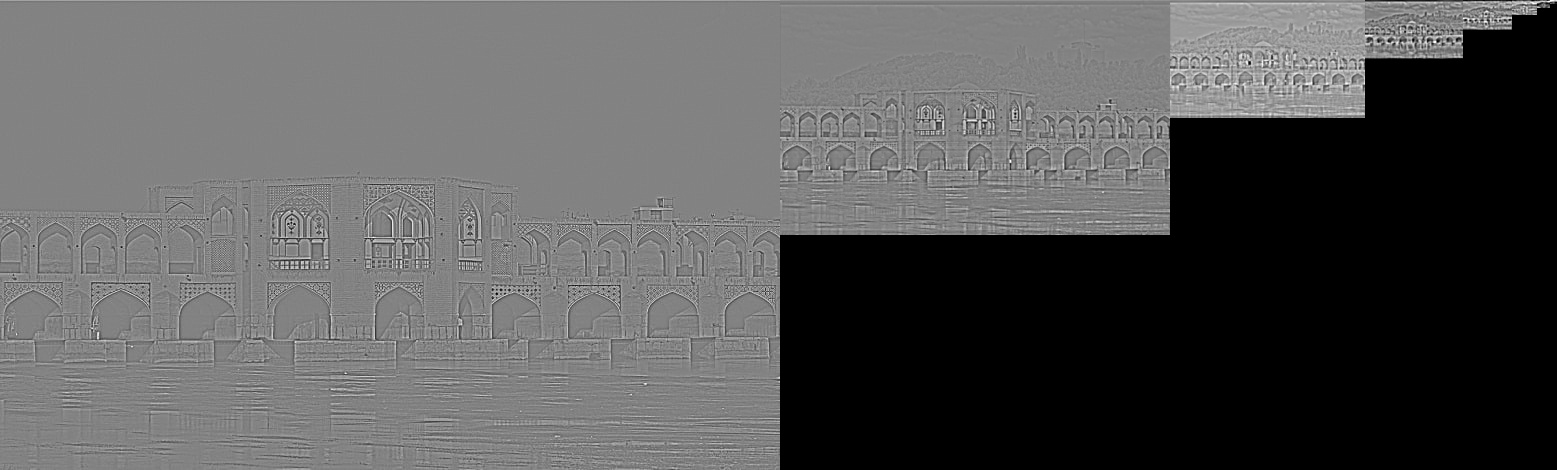
\includegraphics[width=\textwidth]{images/Laplacian_Pyramid_Linear_Set2.jpg}
        \caption{هرم لاپلاسی ترکیبی (مجموعه بناها)}
    \end{subfigure}
    \caption{نتایج نهایی استفاده از ترکیب خطی (فید شدن ملایم فرکانس‌ها کاملاً مشهود است)}
    \label{fig:linear_results}
\end{figure}